\documentclass{article}

\usepackage[utf8]{inputenc}
\usepackage[a4paper, total={6.3in, 8.8in}]{geometry}
\usepackage{amsmath}
\usepackage{bm}
\usepackage{amsfonts}
\usepackage{graphicx}
\usepackage{amssymb}  % assumes amsmath package installed
\usepackage{graphics} % for pdf, bitmapped graphics files
\usepackage{caption}
\usepackage{subcaption}
\usepackage{todonotes}
\usepackage{titling}
\usepackage{float}
\newcommand{\subtitle}[1]{%
  \posttitle{%
    \par\end{center}
    \begin{center}\large#1\end{center}
    \vskip0.5em}%
}

\title{Exercise Session 2: Function Estimation and Time Series Prediction}
\subtitle{Support Vector Machines - Final Report}
\author{Victor van Wymeersch - R0690930}
\date{May 2022}

\begin{document}

\maketitle
    
\section{Exercises} 
    \subsection{Support vector machine for function estimation} 
        This section involves using uiregress to generate a linear dataset to investigate the effects of the hyperparamer e-sensitivity. The e-sensitivity parameter affects the width of the regression tube used to define the support vectors. Large e values correspond to tighter regression or fitting to the datapoints. The tighter the e-bounds the higher the accuracy of fitting and thus more support vectors are needed to make the regression. The phenomenon is illustrated in figure \ref{fig:e-bounds}. For this linear kernel regression when e=0.25, 31 support vectors are needed for linear regression, and when e=0.5, only the two outermost datapoints define the support vectors and thus the regression of the dataset. Larger e-values correspond to models with an increased level of sparsity. 
        % Effect of e 
        \begin{figure}[h]
             \centering
             \hspace{0.05\textwidth}
             % E = small 
             \begin{subfigure}[b]{0.4\textwidth}
                 \centering
                 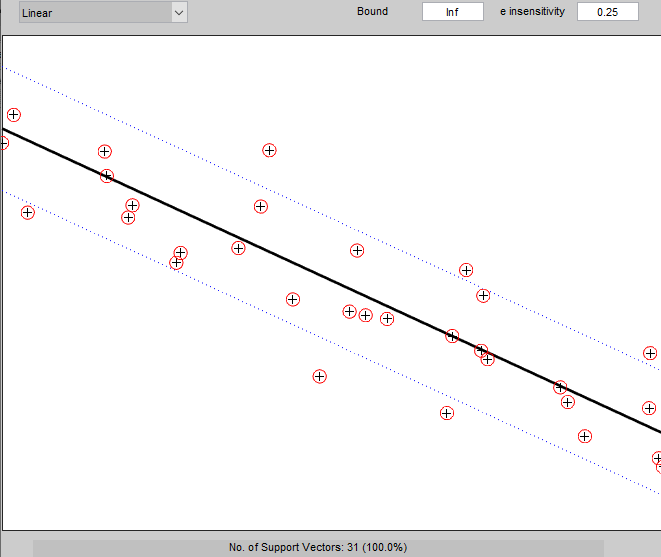
\includegraphics[width=\textwidth]{Assignment 2/figures/1_1/linear_b_inf_e_0_25.png}
                 \caption{e=0.25}
                 \label{fig:linear_small_e}
             \end{subfigure}
             \hfill
            % E = large
             \begin{subfigure}[b]{0.4\textwidth}
                 \centering
                 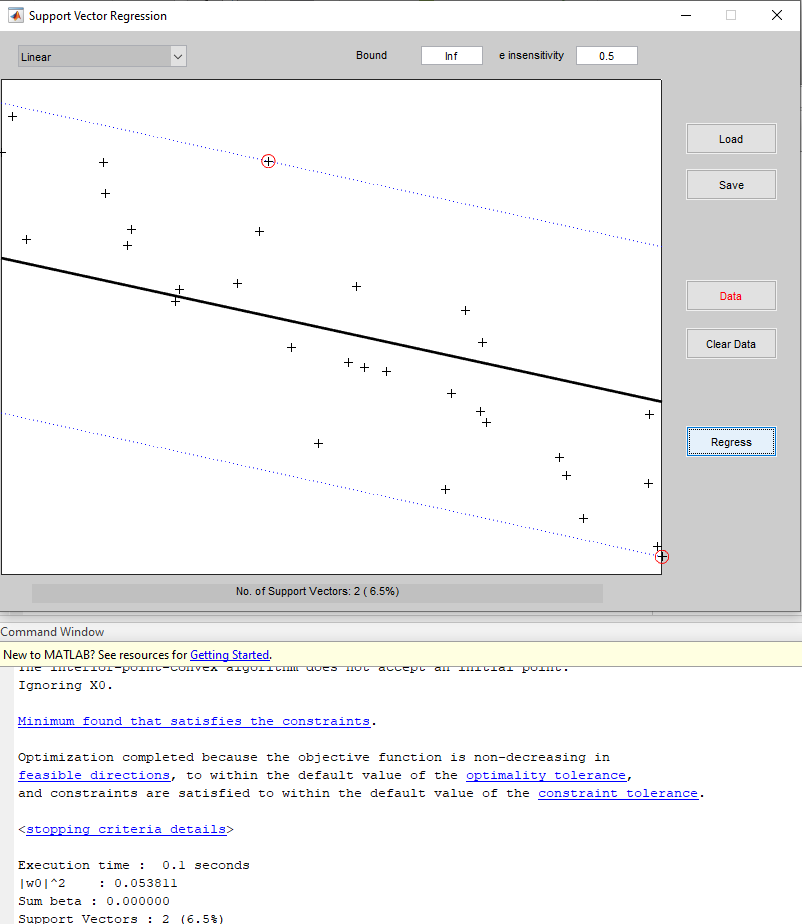
\includegraphics[width=\textwidth]{Assignment 2/figures/1_1/linear_b_inf_e_0_5.png}
                 \caption{e=0.5}
                 \label{fig:linear_large_e}
             \end{subfigure}
             \hspace{0.05\textwidth}
            \caption{Linear classification boundary in response to different values of e. }
            \label{fig:e-bounds}
        \end{figure}
        
        % \begin{enumerate}
        %     \item e small: $|w0|^2$ =0.38, beta=0.01
        %     \item e large: $|w0|^2$ = 0.05, beta=0.00
        % \end{enumerate}
    
        The second parameter investigated is the bound. For this a RBF kernel is used on another linear dataset as this most clearly illustrates the effect of the parameter. The dataset is shown in figure \ref{fig:bound_effect}. When the bound equals 0.05 the result is a model that under fits the data as shown in figure \ref{fig:rbf_small_bound}. When looking at the objective function being solved in this regression problem:
        \begin{equation}\label{eq:bound}
        \begin{split}
            \min_{w,b,\xi} & \ \frac{1}{2} w^T w + C \sum^N_{k=1} \xi_k,
        \end{split}
        \end{equation}
        we see that for larger bounds the slack variables $\xi_k$ dominate the optimisation problem. When larger bound values are chosen, equal to 10, we are able to correctly regress the data with a near linear line. This corresponds to a good balance between minimising both $w^T w$ and $\sum^N_{k=1} \xi_k$ terms in the objective function, not over- or under-fitting the data. When the bound is increased even further to 10000, we over-fit the data and lose the linear regression line obtained before. 
        % Effect of bound on RBF classification linear 
        \begin{figure}[h]
             \centering
             % bound small - underfitting 
             \begin{subfigure}[b]{0.3\textwidth}
                 \centering
                 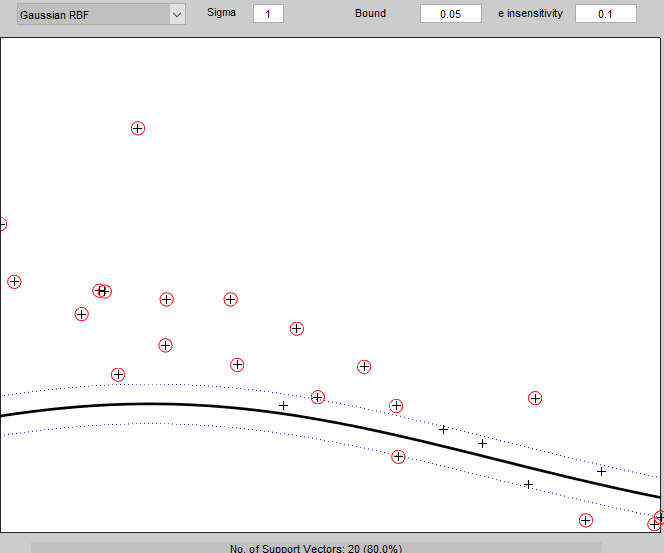
\includegraphics[width=\textwidth]{Assignment 2/figures/1_1/rbf_bound_small.png}
                 \caption{Under-fitting ($bound=0.05$)}
                 \label{fig:rbf_small_bound}
             \end{subfigure}
             \hfill
             % bound medium - fitted 
             \begin{subfigure}[b]{0.3\textwidth}
                 \centering
                 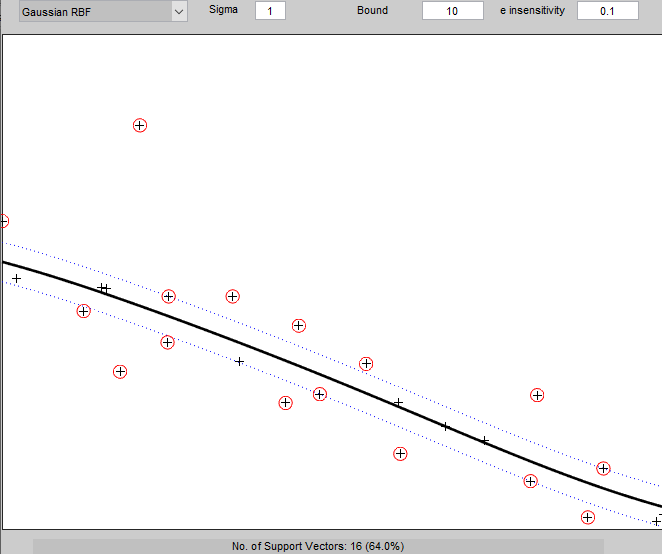
\includegraphics[width=\textwidth]{Assignment 2/figures/1_1/rbf_bound_medium.png}
                 \caption{Correctly fitted ($bound=10$)}
                 \label{fig:rbf_medium_bound}
             \end{subfigure}
             \hfill
             % bound large - over-fitted  
             \begin{subfigure}[b]{0.3\textwidth}
                 \centering
                 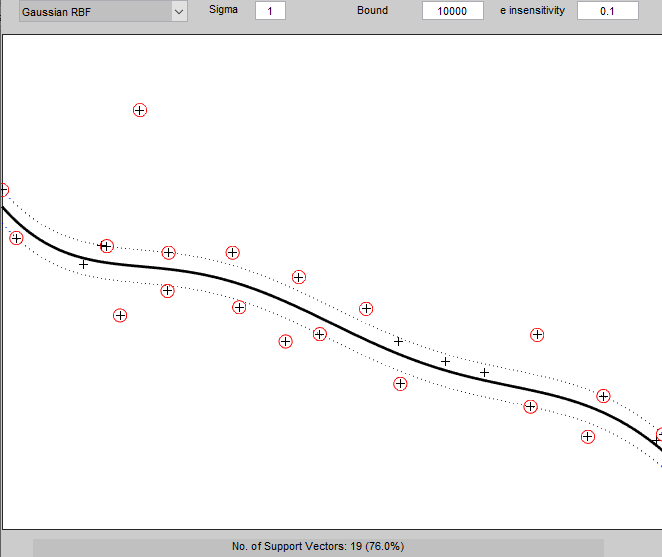
\includegraphics[width=\textwidth]{Assignment 2/figures/1_1/rbf_bound_large.png}
                 \caption{Over-fitting ($bound=10000$)}
                 \label{fig:rbf_large_bound}
             \end{subfigure}
            \caption{Effect of varying bound for regression on a linear dataset using a RBF kernel.}
            \label{fig:bound_effect}
        \end{figure}
        
        % \begin{enumerate}
        %     \item Under: $|w0|^2$ = 0.42, beta=0.64
        %     \item proper: $|w0|^2$ = 2.34, beta=1.57
        %     \item over:$|w0|^2$ = 303.97, beta=6.79
        % \end{enumerate}
        
        When fitting to a nonlinear dataset with a wavy structure, as shown in figure \ref{fig:gauss_rbf}. Here we require a nonlinear model to properly regress the data and thus, a Gaussian RBF kernel is used with $\sigma=0.2$, bound$=2$, and $e=0.1$. 
        % Nonlinear dataset
        \begin{figure}[h]
             \centering
            % RBF kernel 
             \centering
             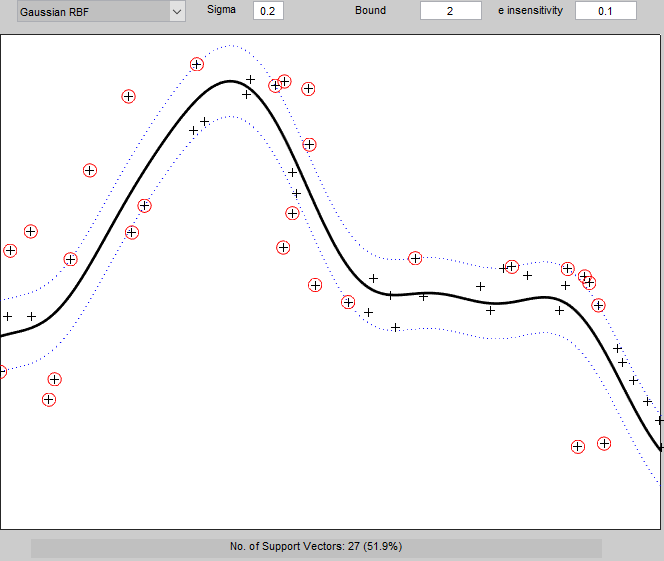
\includegraphics[width=0.5\textwidth]{Assignment 2/figures/1_1/gauss_rbf_sig_0_2_b_2_e_0_1.png}
            \caption{Regression results for Gaussian RBF kernels on a nonlinear dataset.}
            \label{fig:gauss_rbf}
        \end{figure}
        
        % \begin{enumerate}
        %     \item guass rbf: $|w0|^2$ =1.89, beta=2.43
        % \end{enumerate}
    
        The difference between SVM regression and the classical least squares regression lies in the loss functions. The loss function of SVM is defined by Vapnik's e-insensitive loss function, which tolerates small errors between $-e$ and $e$ and acts as an L1 loss outside these values. On the contrary a classical least squares regression problem utilizes the L2 loss function across the whole input domain. Moreover, SVM enables the use of various non-linear kernels, adding flexibility in the way regression can be performed.
    
    \subsection{A simple example: the sinc function}
        In this section we perform least squares SVM regression on the simple Sinc function using a RBF kernel.
        
        \subsubsection{Regression of the sinc function}
            Several different values for $\gamma$ and $\sigma^2$ were tested and the Root Mean Squared Errors (RMSE) on the test set were plotted as illustrated in figure \ref{fig:gauss_rbf_tuned}. 
            % Manual tuning of hyperparameters 
            \begin{figure}[h]
                 \centering
                 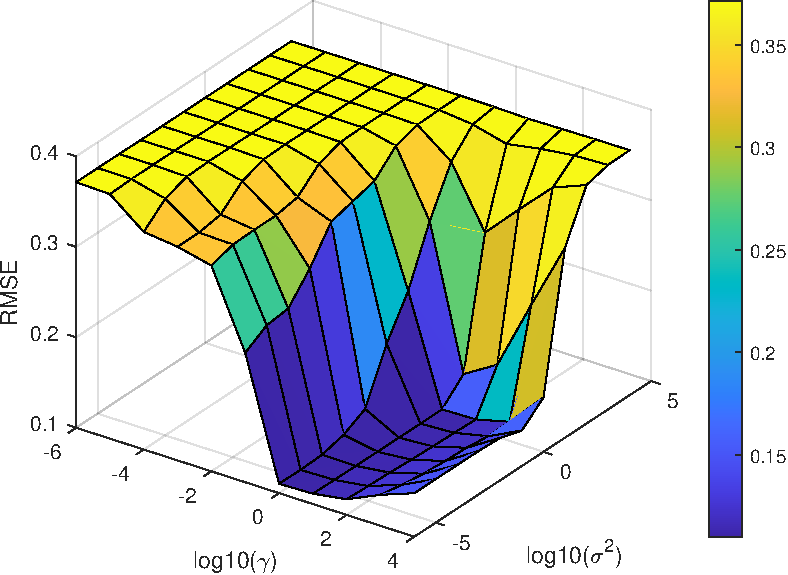
\includegraphics[width=0.6\textwidth]{Assignment 2/figures/1_2/hyper_tuning_results.pdf}
                 
                \caption{RMSE for varying $\sigma^2$ and $\gamma$ hyperparameters during regression of the Sinc function.}
                \label{fig:gauss_rbf_tuned}
            \end{figure}
            
            We can see that when the regularisation parameter $\gamma$ is taken too low, the RMSE rises dramatically fails to  properly reduce the fitting-error on the dataset. Additionally we can see that when $\sigma^2$ is taken too high then the RMSE also rises because the model does not have enough flexibility to fit the Sinc function. For very low values of $\sigma^2$ and very high values of $\gamma$ it seems that the model manages a very low RMSE, however when looking at figures \ref{fig:high_gamma} and \ref{fig:low_sigma}, we see that in these cases the models simply overfit the data to obtain low RMSEs and do not smoothly fit the data.  
            
            % tuning results
            \begin{figure}[h]
                 \centering
                 \hspace{0.05\textwidth}
                 \begin{subfigure}[b]{0.4\textwidth}
                     \centering
                     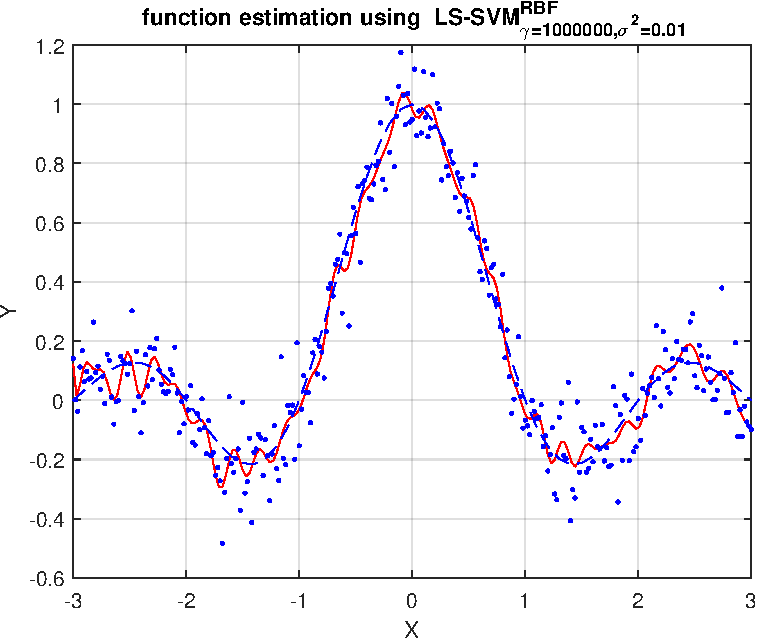
\includegraphics[width=\textwidth]{Assignment 2/figures/1_2/rbf_reg_sig2_0.01_gam_1000000.00.pdf}
                     \caption{$\sigma^2=0.01,\ \gamma=1000000$}
                     \label{fig:high_gamma}
                 \end{subfigure}
                 \hfill
                 \begin{subfigure}[b]{0.4\textwidth}
                     \centering
                     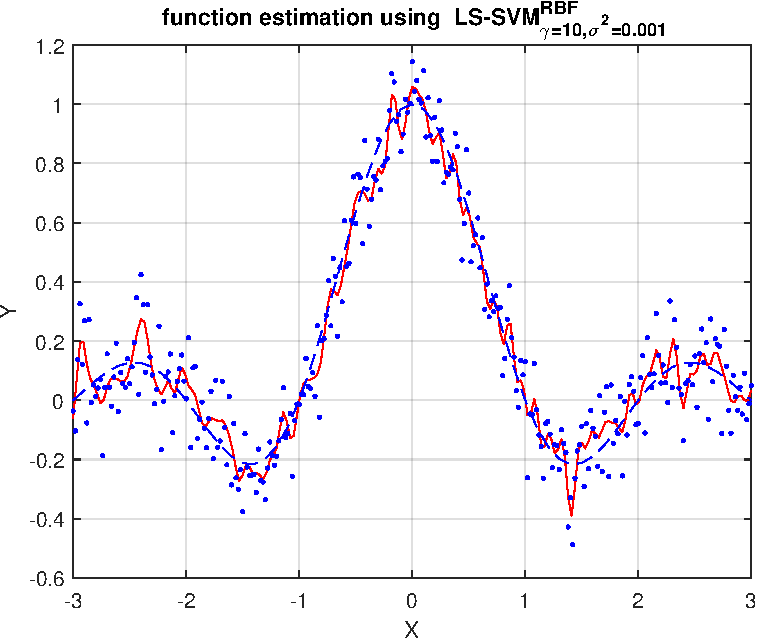
\includegraphics[width=\textwidth]{Assignment 2/figures/1_2/rbf_reg_sig2_0.00_gam_10.00.pdf}
                     \caption{$\sigma^2=0.001,\ \gamma=10$}
                     \label{fig:low_sigma}
                 \end{subfigure}
                \hspace{0.05\textwidth}
                \caption{Effects of $\sigma^2$ on the regression results.}
            \end{figure}
            
            After tuning the regression hyperparameters with the Simplex and Gridsearch parameters the following parameters were obtained: 
            \begin{table}[H]
            \centering
            \begin{tabular}{|c|c|c|}
            \hline
            \textbf{}           & \textbf{Simplex} & \textbf{Gridsearch} \\ \hline
            \textbf{$\gamma$}   & \textbf{8.82}    & \textbf{36422}      \\ \hline
            \textbf{$\sigma^2$} & \textbf{0.22}    & \textbf{0.91}       \\ \hline
            \textbf{RMSE}       & \textbf{0.11}    & \textbf{0.11}       \\ \hline
            \end{tabular}
            \end{table}
            
            With these tuned hyperparameters smooth properly fitted function can be observed as illustrated in figure \ref{fig:smooth}.
            The Simplex and Gridsearch tuning algorithms were run multiple times receiving near near identical RMSEs and good fitting results with different hyperparameters. This confirms that there is no single set of optimal parameters but rather a set of hyperparameter combinations that properly fit the problem at hand, as a result of the many local minima that exist in the optimisation problem considered. 
             % Simplex and Gridsearch tuning results
            \begin{figure}[h]
                 \centering
                 \hspace{0.05\textwidth}
                 % simplex
                 \begin{subfigure}[b]{0.4\textwidth}
                     \centering
                     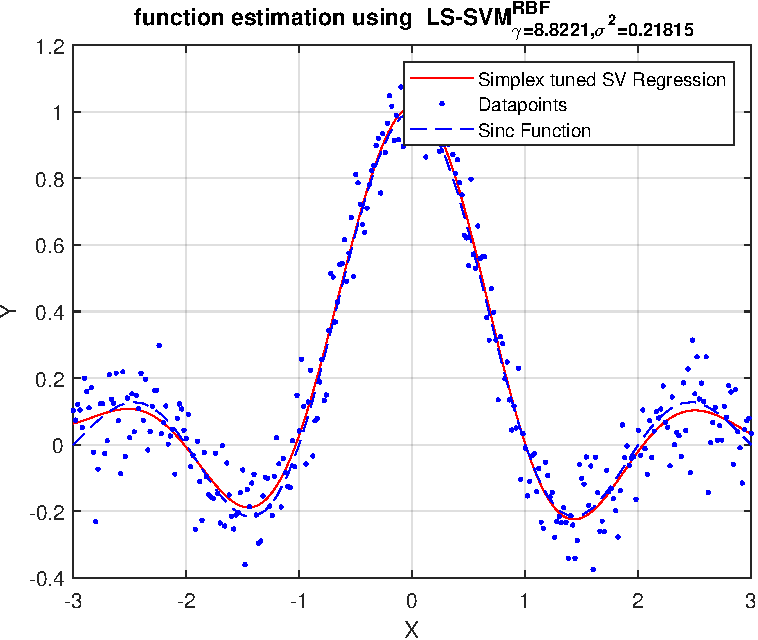
\includegraphics[width=\textwidth]{Assignment 2/figures/1_2/rbf_tuning_results_simp.pdf}
                     \caption{Simplex}
                     \label{fig:regression_simplex_tuned}
                 \end{subfigure}
                 \hfill
                % gridsearch
                 \begin{subfigure}[b]{0.4\textwidth}
                     \centering
                     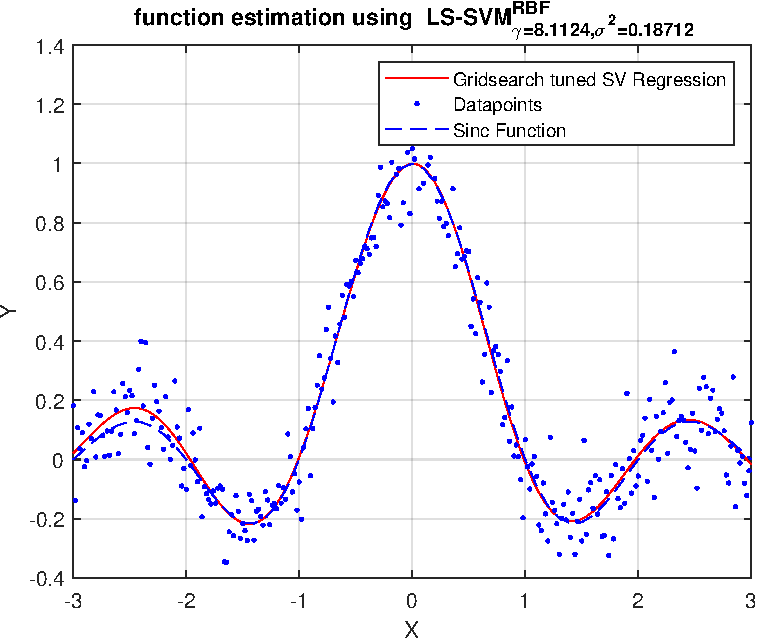
\includegraphics[width=\textwidth]{Assignment 2/figures/1_2/rbf_tuning_results_grid.pdf}
                     \caption{Gridsearch}
                     \label{fig:regression_grisearch_tuned}
                 \end{subfigure}
                 \hspace{0.05\textwidth}
                \caption{Regression on the Sinc function with RBF kernel tuned with hyperparameters tuned with different algorithms.}
                \label{fig:smooth}
            \end{figure}
            
        \subsubsection{Application of the Bayesian framework}
        In this section the Bayesian framework for optimal tuning of hyperparameters is investigated. Fundamentally the Bayesian framework relies on the derivation of the probability that the data points are generated by the given model, or the posterior probability. During this tuning approach three levels are considered: 
        
        \begin{itemize}
            \item Step 1: The posterior optimisation with respect to the support $\alpha$ and bias $b$ terms.
            \item Step 2: The posterior optimisation with respect to the regularisation constant $\gamma$.
            \item Step 3: The posterior optimisation with respect to the choice of the kernel and its associated hyperparameters ($\sigma^2$ for the RBF kernel).
        \end{itemize}
        
        The optimisation is formulated as follows: 
        \begin{equation}\label{eq:bayestuning}
        \begin{split}
            \min_{w,b,e} & \  J_p(w,e) = \mu E_W + \zeta E_D \\
            \text{s.t.} & \   y_k = w^T \varphi(x_k) + b + e_k,
        \end{split}
        \end{equation}
        for $k=1,...,N$, where $E_w = \frac{1}{2} w^Tw$ and $E_D = \frac{1}{2} \sum^N_{k=1} e_k^2$. 
        
        Through the minimisation of the optimisation problem the posterior is maximised for the dataset. The results for such an optimisation of the hyperparameters through the Bayesian framework, and applied to the Sinc function is shown in figure \ref{fig:bayesianregression_sinc}. Here $\gamma$ is determined as $0.46087$ and $\sigma^2$ as $0.23115$, resulting in near perfect fit to the data. The figure also shows the $2\sigma$ confidence bounds associated with the regression, a strong benefit of the Bayesian framework. 
            % Bayesian framework for parameter tuning and regression 
            \begin{figure}[h]
                 \centering
                 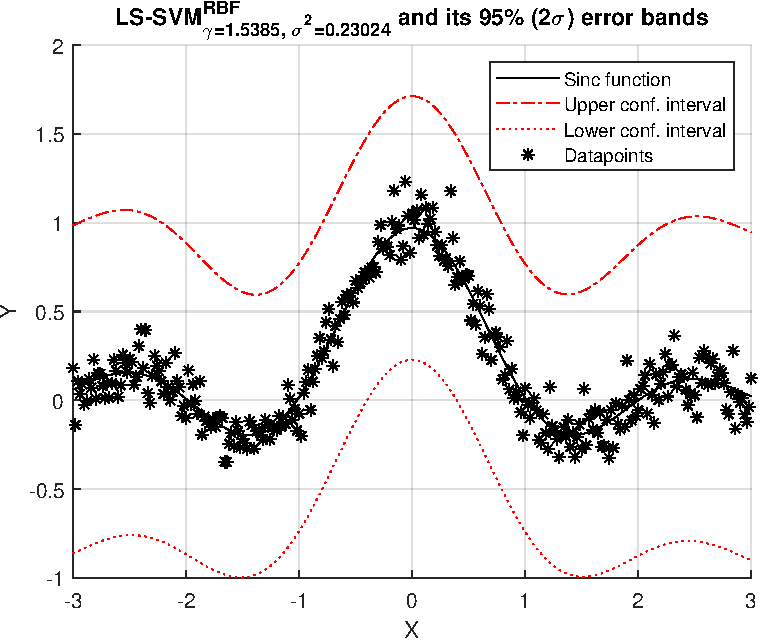
\includegraphics[width=0.5\textwidth]{Assignment 2/figures/1_2/bayesian_regression.pdf}
                \caption{Bayesian SVM regression of the Sinc function. }
                \label{fig:bayesianregression_sinc}
            \end{figure}
        
    \subsection{Automatic Relevance Determination}
        A secondary benefit to the Bayesian framework is that it can also be used to select the most relevant inputs in a set of data through Automatic Relevance Determination (ARD). To determine the most relevant input the method uses backward selection to eliminate features one-by-one by assigning a $\sigma^2$ weighting parameter to each dimension. By optimising the $\sigma^2$ parameter, the inputs with the largest $\sigma^2$ values are removed. 
        
        The ARD algorithm is applied to a three dimensional input, with one of the dimensions being the Sinc function. Though the backward selection process ARD finds and fits to the Sinc function. The results are displayed in figure \ref{fig:bayesianregression_ard}. ARD performs well on this dataset as it only has 3 features, however the time complexity is exponential with  the number of input features and cannot be used on data with high dimensionality unless prepossessing like PCA is performed. 
        
        % ARD
        \begin{figure}[h]
             \centering
             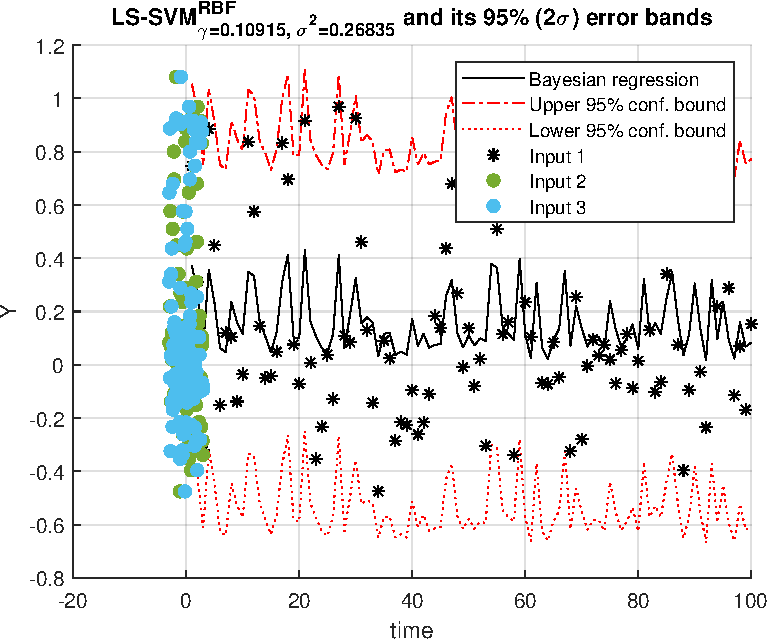
\includegraphics[width=0.5\textwidth]{Assignment 2/figures/1_3/bayesian_regression.pdf}
            \caption{Automatic relevance determination using the Bayesian framework.}
            \label{fig:bayesianregression_ard}
        \end{figure}
        
        Contrasting to ARD, input selection can also be performed using cross-validation through Recursive Feature Elimination. This method ranks features according to the weights learned during regression. Weak features are discarded one by one and the model is retrained with the reduced feature set. Performance on the reduced feature set is evaluated using cross validation. If the performance suffers as a result of removing a feature, the feature is established as important and kept. The process is repeated until only the most relevant features remain. 
            
            
    \subsection{Robust regression}
        Many datasets contain outliers or non-Gaussian noise which make regression difficult. In these cases it becomes important to incorporate robustness schemes into estimations. In this section we add outliers to the Sinc dataset and perform standard LS-SVM regression and robust LS-SVM regression. The results of the standard and robust regression are displayed in figures \ref{fig:non_robust_regression} and \ref{fig:robust_regression}, respectfully. It is clear from figure \ref{fig:non_robust_regression}, that in the presence of outliers the performance of the model deteriorates when compared to figure \ref{fig:robust_regression}. In standard LS-SVM regression outliers get squared in the LS loss function, causing a strong influence on the result of the regression. For this reason, the Mean Absolute Error (MAE) or L1-norm is often preferred over the standard MSE L2-norm because of its robustness to outliers.   
        
        
        % Robust vs nonrobust regression 
        \begin{figure}[h]
             \centering
             \hspace{0.05\textwidth}
             % robust
             \begin{subfigure}[b]{0.4\textwidth}
                 \centering
                 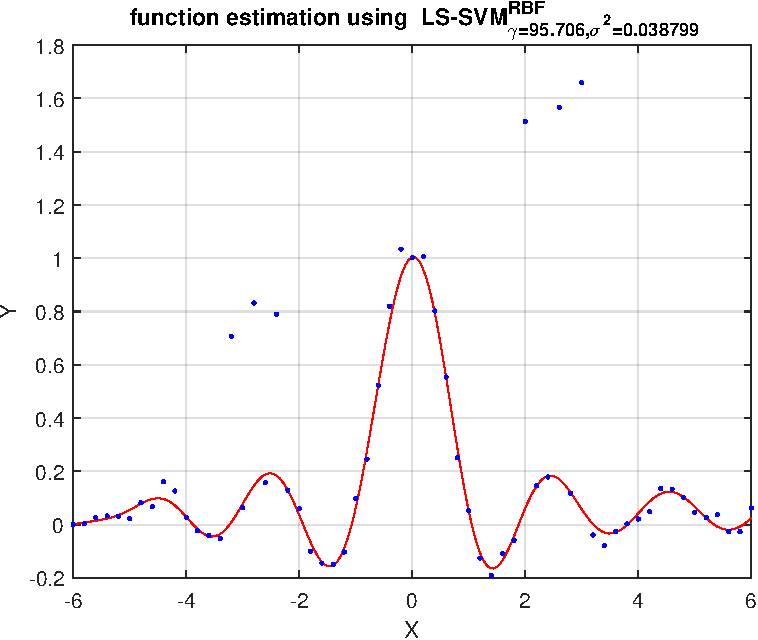
\includegraphics[width=\textwidth]{Assignment 2/figures/1_4/robust_mae_whuber.pdf}
                 \caption{Robust regression}
                 \label{fig:robust_regression}
             \end{subfigure}
             \hfill
            % Non robust
             \begin{subfigure}[b]{0.4\textwidth}
                 \centering
                 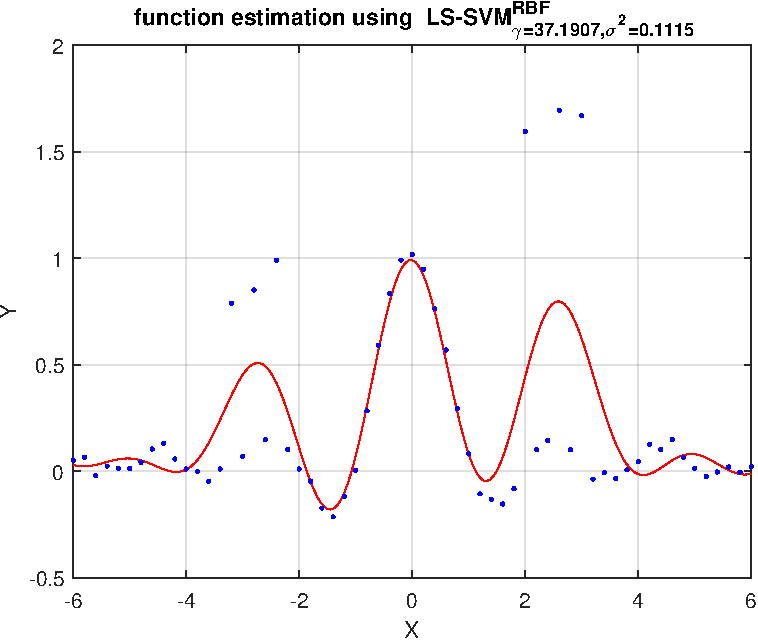
\includegraphics[width=\textwidth]{Assignment 2/figures/1_4/standard_mse.pdf}
                 \caption{Non-robust regression}
                 \label{fig:non_robust_regression}
             \end{subfigure}
             \hspace{0.05\textwidth}
            \caption{Robust vs non-robust regression in the presence of noise on the Sinc function. }
        \end{figure}
        
        Robust regression problems are formulated as follows: 
        \begin{equation}\label{eq:robust_regression}
            \min_{w,b,e_k} \ \frac{1}{2} w^T w + \gamma \sum^N_{k=1} v_k e_k^2, 
        \end{equation}
        where $v_k$ represents the weight applied to every instance of the dataset. The weights $v_k$ are determined though weighting functions such as Huber, Hampel, Myriad, or Logistic. Depending on the choice of the weighting function, different outlier rejection capabilities are obtained. The results of Huber, Hampel, Myriad, or Logistic weighting functions for robust regression are illustrated in figures \ref{fig:robust_regression_huber}, \ref{fig:robust_regression_hampel}, \ref{fig:robust_regression_myriad}, and \ref{fig:robust_regression_logistic}, respectfully. For this dataset all weighting functions perform almost identically. 
        % Robust regression function comparison
        \begin{figure}[h]
             \centering
             % huber
             \begin{subfigure}[b]{0.22\textwidth}
                 \centering
                 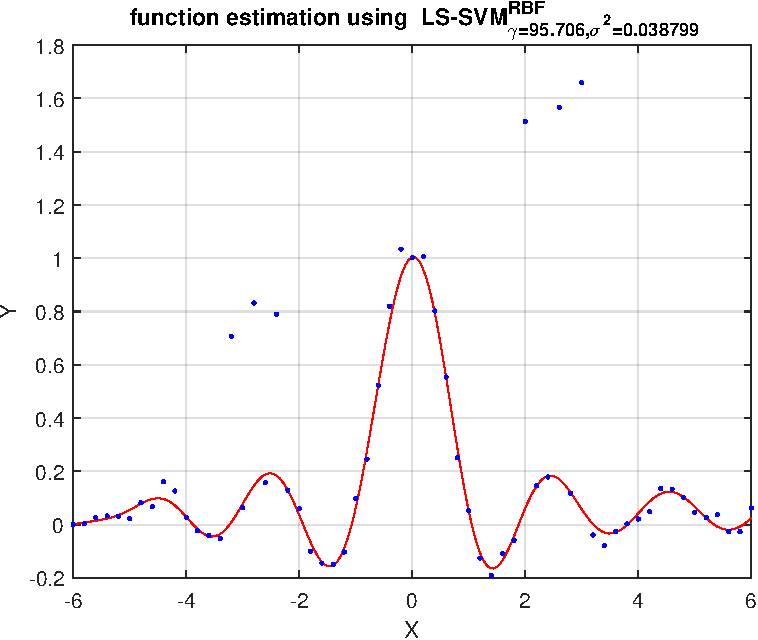
\includegraphics[width=\textwidth]{Assignment 2/figures/1_4/robust_mae_whuber.pdf}
                 \caption{Huber}
                 \label{fig:robust_regression_huber}
             \end{subfigure}
             \hfill
             %hampel
            \begin{subfigure}[b]{0.22\textwidth}
                 \centering
                 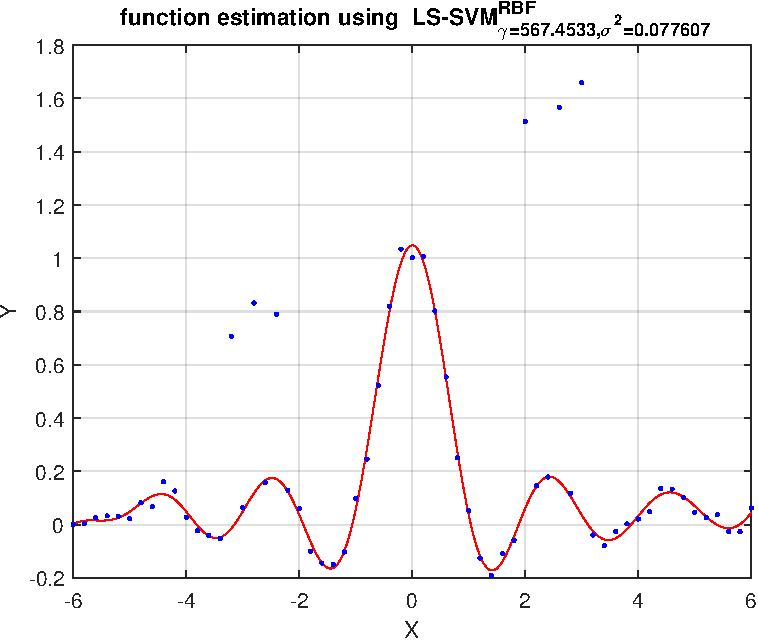
\includegraphics[width=\textwidth]{Assignment 2/figures/1_4/robust_mae_whampel.pdf}
                 \caption{Hampel}
                 \label{fig:robust_regression_hampel}
             \end{subfigure}
             \hfill
             %myriad
             \begin{subfigure}[b]{0.22\textwidth}
                 \centering
                 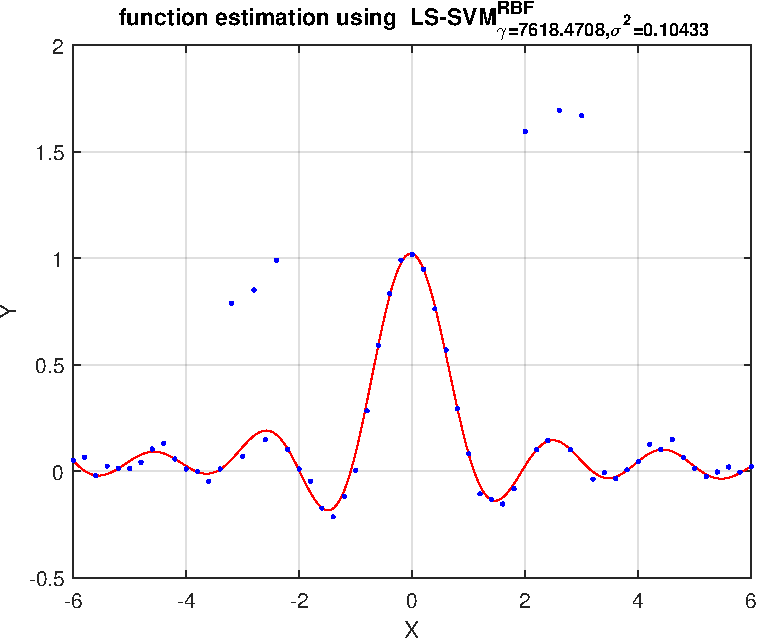
\includegraphics[width=\textwidth]{Assignment 2/figures/1_4/robust_mae_wmyriad.pdf}
                 \caption{Myriad}
                 \label{fig:robust_regression_myriad}
             \end{subfigure}
             \hfill
             %logistic
             \begin{subfigure}[b]{0.22\textwidth}
                 \centering
                 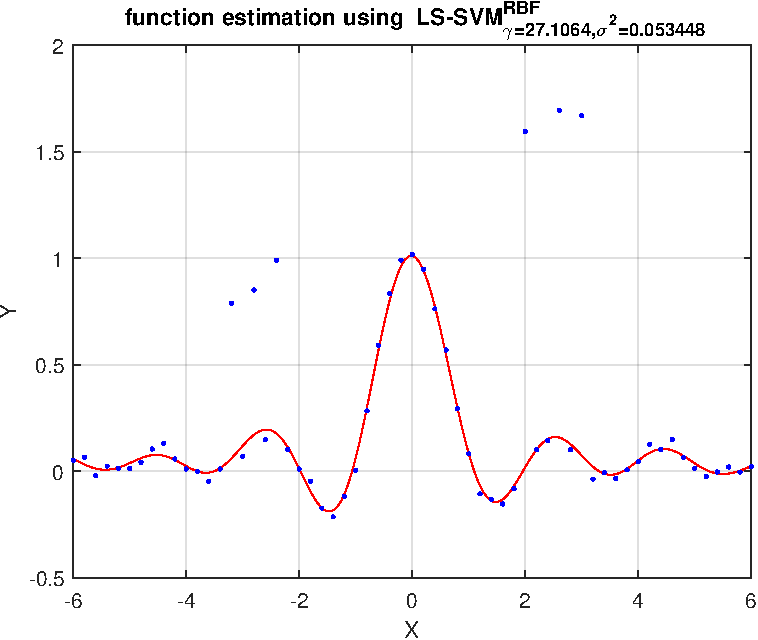
\includegraphics[width=\textwidth]{Assignment 2/figures/1_4/robust_mae_wlogistic.pdf}
                 \caption{Logistic}
                 \label{fig:robust_regression_logistic}
             \end{subfigure}
            \caption{Robust regression results for different weighting functions.}
        \end{figure}
    
\section{Homework problems}
    \subsection{Introduction: time series prediction}
        In this section we investigate the effect of different parameters for LS-SVM for in predicting unseen time-series data. This Auto Regressive (AR) problem consists of finding a nonlinear mapping (f) approximate: 
        \begin{equation}
            \hat{y}_t = f(x_t), 
        \end{equation}
        where the targets are future data points $y_t = z_t$, and input features are past datapoints $x_t=[z_{t-1}, z_{t_2}, ... ,  z_{t-n}]'$. Here $n$ represents the order of the problem, or alternatively how many datapoints to utilise for a prediction. 
        
    \subsection{Logmap dataset}
        In this section AR time series prediction on the Logmap dataset is performed over 50 future timesteps. To do so three parameters are optimised, namely: the order, $\sigma^2$ and $\gamma$. $\sigma^2$ and $\gamma$ are Simplex-tuned using 10-fold cross validation, and the order is tuned through a parameter sweep between the following values: \newline $[1, 3, 5, 10, 20, 30, 40, 50, 60, 70, 80, 90, 100]$.
         For each order the MSE and MAE errors are calculated to establish the best combination of hyperparameters to accurately predict future values on the test set. The result of the order parameter sweep is shown in figure \ref{fig:order_sweep}. The best performing hyperparameters were: 
        \begin{itemize}
            \item $\gamma =  42.56$
            \item $\sigma^2 =  2105.75$
            \item Order$= 50$
        \end{itemize}
        
        Figure \ref{fig:logmap_prediction} shows the prediction result on the test set for a resulting RMSE of $0.2244$. It can be seen that for some parts of the dataset the predictions perform very well, such as between samples 23-30 and 43-48. However, some predictions are out of phase or do not correspond to the magnitude of the test sets values.
        % Time series prediction logmap
        \begin{figure}[h]
             \centering
             \hspace{0.05\textwidth}
             % Order tuning
             \begin{subfigure}[b]{0.4\textwidth}
                 \centering
                 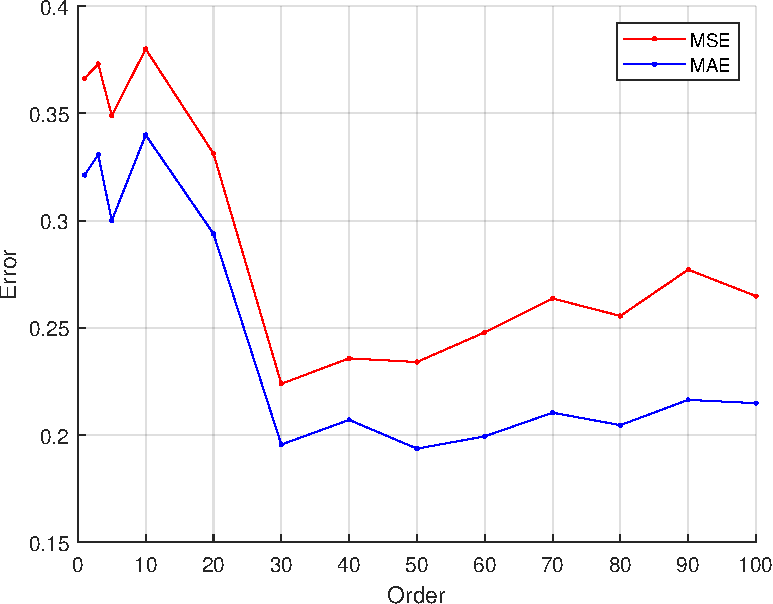
\includegraphics[width=\textwidth]{Assignment 2/figures/2_2/MSEvsMAE_ordersweep.pdf}
                 \caption{Errors for different orders.}
                 \label{fig:order_sweep}
             \end{subfigure}
             \hfill
             \begin{subfigure}[b]{0.4\textwidth}
                 \centering
                 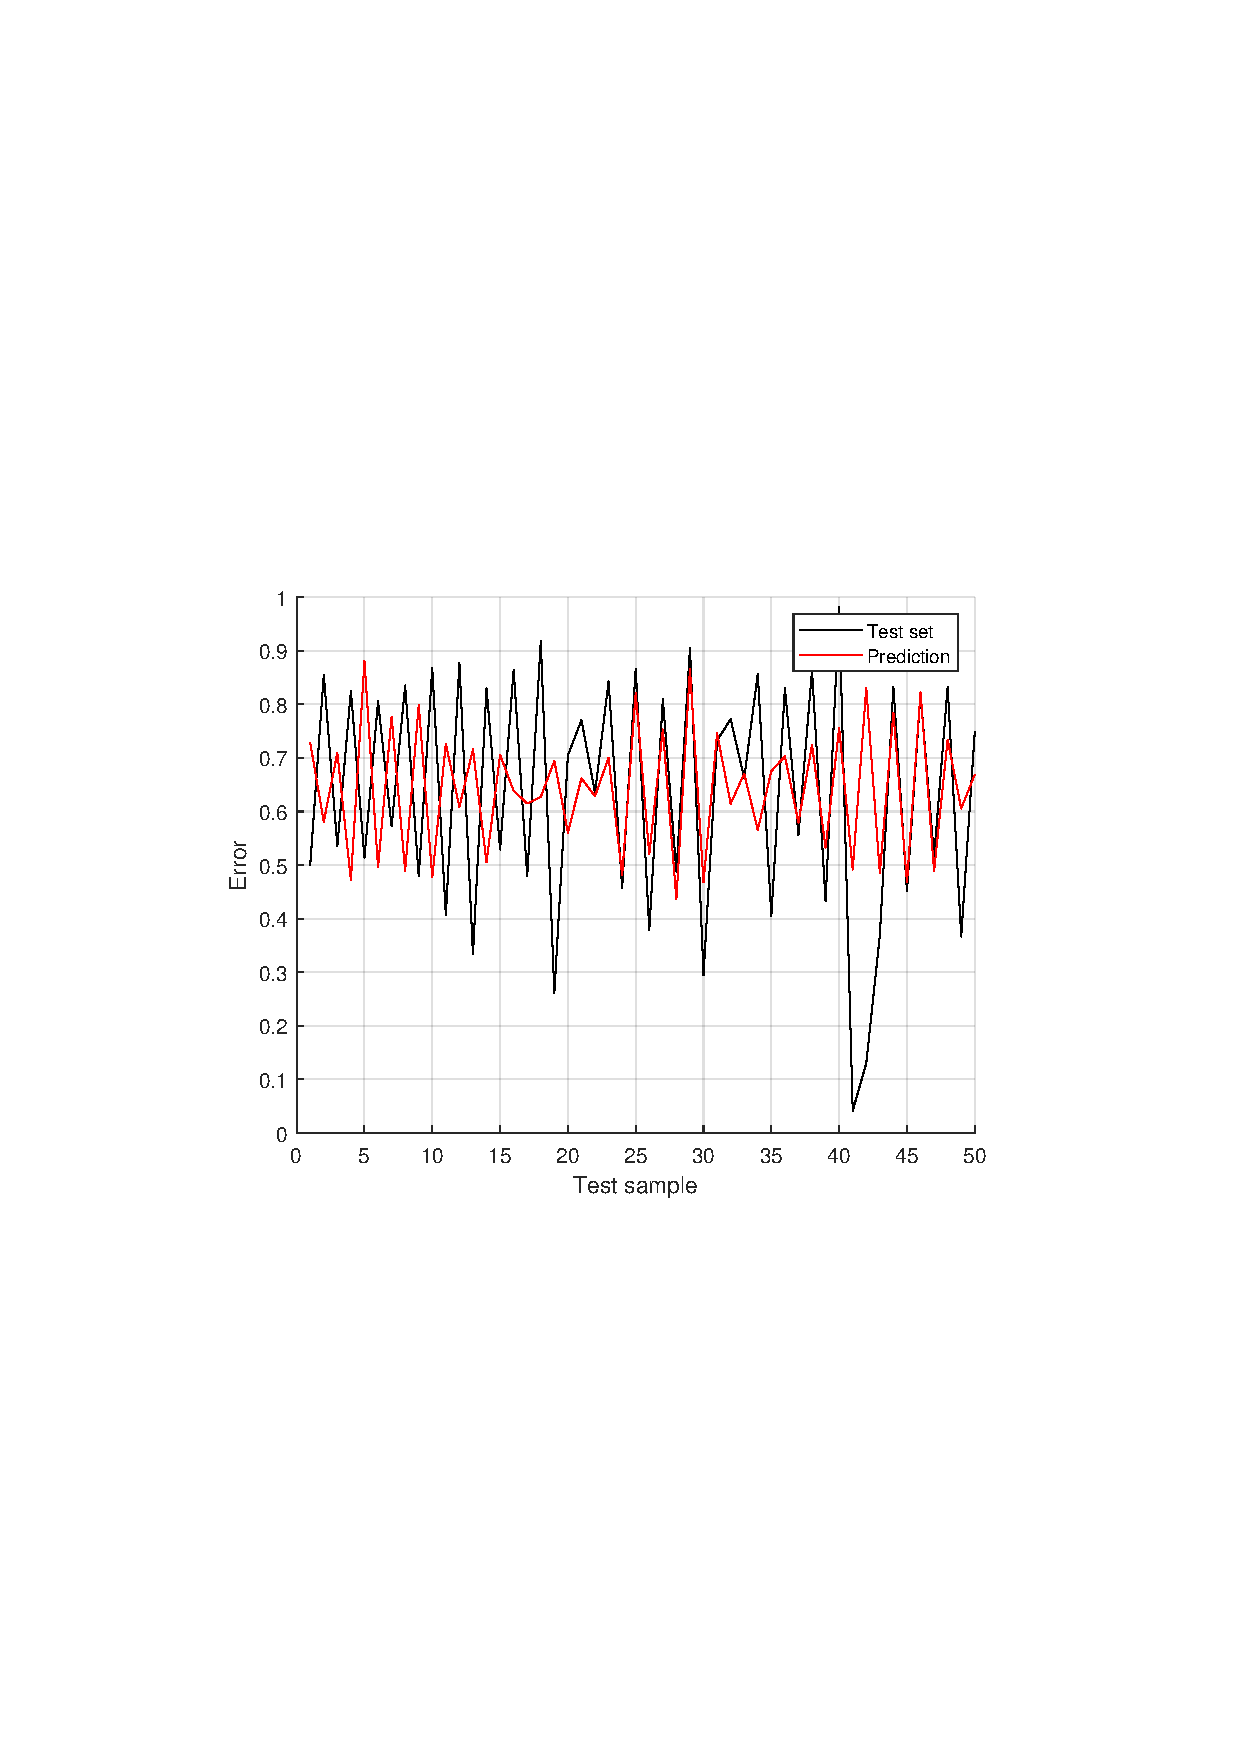
\includegraphics[width=\textwidth]{Assignment 2/figures/2_2/prediction.pdf}
                 \caption{Time series prediction result.}
                 \label{fig:logmap_prediction}
             \end{subfigure}
             \hspace{0.05\textwidth}
            \caption{Tuning (a) and prediction (b) results for time series regression on the Logmap dataset.}
        \end{figure}
        
    \subsection{Santa Fe dataset}
        In this section AR time series prediction on the Santa Fe dataset is performed over 200 future timesteps. The first investigation is in evaluating order=50 for an AR model on the Santa Fe dataset. For this task $\sigma^2$ and $\gamma$ are also Simplex-tuned using 10-fold cross validation. The performance of the model does poorly on the test set as can be seen on figure \ref{fig:order_50}. With an order of 50 the model only has very little information about the change in amplitude of the time series data and thus results in an inability to predict the drop. 
        \begin{figure}[h]
             \centering
             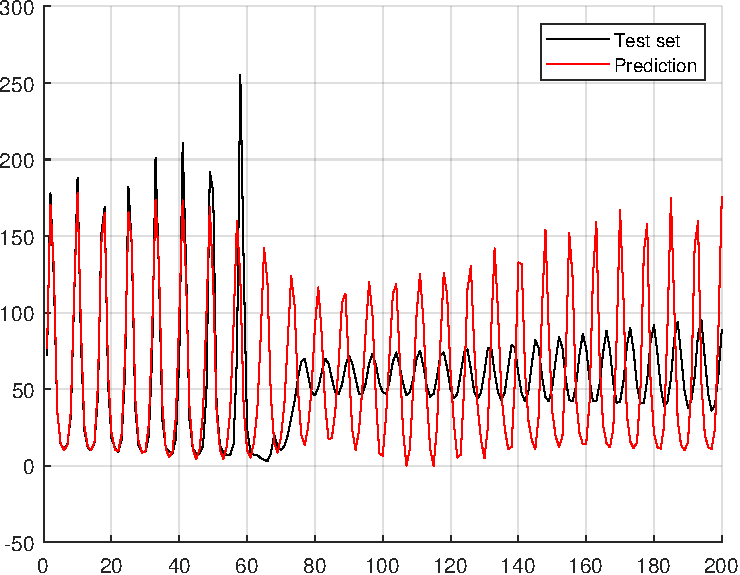
\includegraphics[width=0.5\textwidth]{Assignment 2/figures/2_3/order50.pdf}
            \caption{Time series prediction result for order = 50. }
            \label{fig:order_50}
        \end{figure}
        
        
        To obtain a better result three parameters need to be optimised, namely: the order, $\sigma^2$ and $\gamma$. $\sigma^2$ and $\gamma$ are Simplex-tuned using 10-fold cross validation, and the order is tuned through a parameter sweep between the following values: \newline $[5, 10, 20, 30, 50, 70, 100, 300]$.
         For each order the MSE and MAE errors are calculated to establish the best combination of hyperparameters to accurately predict future values on the test set. The result of the order parameter sweep is shown in figure \ref{fig:order_sweep_santa_fe}. The best performing hyperparameters were: 
        \begin{itemize}
            \item $\gamma =  3200.30$
            \item $\sigma^2 =  14.65$
            \item Order$= 30$
        \end{itemize}
        
        Figure \ref{fig:santafe_prediction} shows the prediction result on the test set for a resulting RMSE of $19.22$. The model's predictions perform very well on the first dozen time steps, however goes out of phase with the test set after test sample number 70.
        
        % Time series prediction Santa Fe
        \begin{figure}[h]
             \centering
             \hspace{0.05\textwidth}
             % Order tuning
             \begin{subfigure}[b]{0.4\textwidth}
                 \centering
                 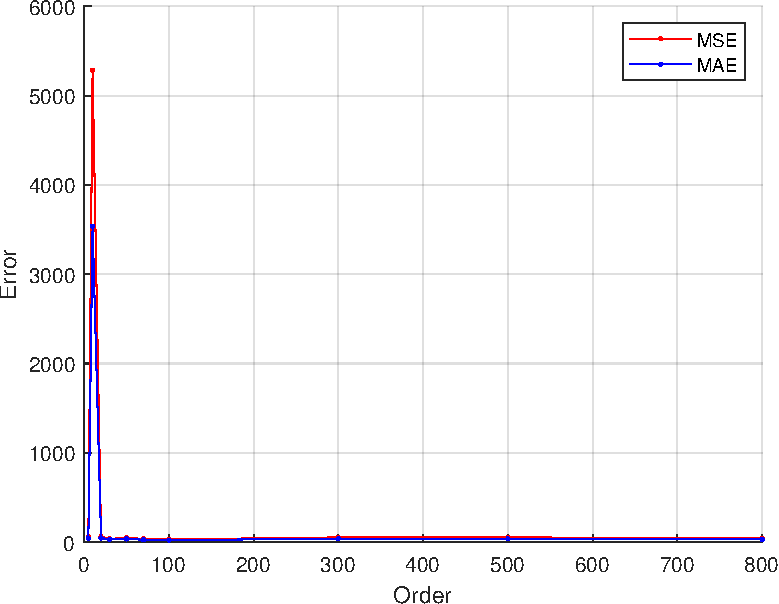
\includegraphics[width=\textwidth]{Assignment 2/figures/2_3/MSEvsMAE_ordersweep.pdf}
                 \caption{Errors for different orders.}
                 \label{fig:order_sweep_santa_fe}
             \end{subfigure}
             \hfill
            % Non robust
             \begin{subfigure}[b]{0.4\textwidth}
                 \centering
                 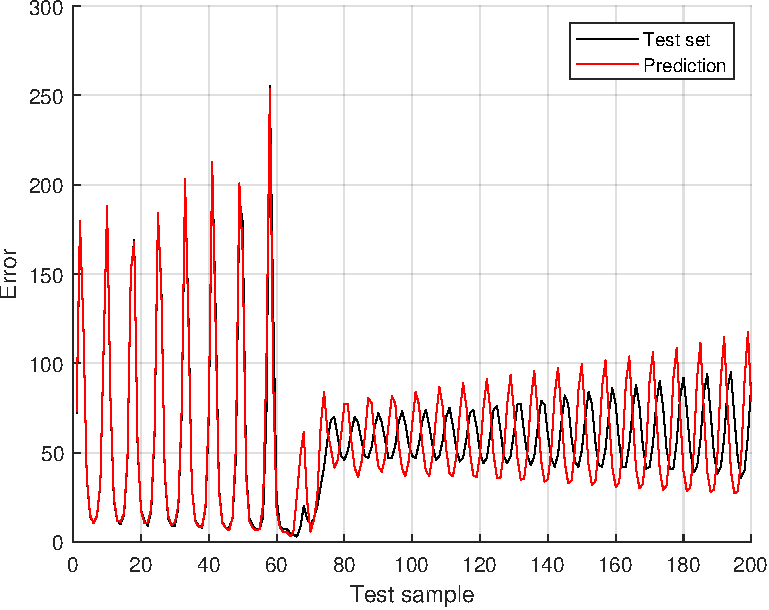
\includegraphics[width=\textwidth]{Assignment 2/figures/2_3/prediction_order_20.pdf}
                 \caption{Time series prediction result.}
                 \label{fig:santafe_prediction}
             \end{subfigure}
             \hspace{0.05\textwidth}
            \caption{Tuning (a) and prediction (b) results for time series regression on the Santa Fe dataset.}
        \end{figure}
        
    


\end{document}